\documentclass[12pt]{article}

\usepackage[spanish,activeacute]{babel}
\usepackage{amsmath}
\usepackage{graphicx}

\title{Reto 1}
\author{Jorman Bustos - Topicos avanzados en telematica}

\begin{document}
\maketitle

%autores
%requerimientos
%como ejecutar cliente y server

\section{Enunciado}
Se parte de una aplicación llamada “calculadora”, la cual permite e implementa cuatro (4) operaciones basicas: Restar, Multiplicar, Dividir,
a nivel de funcionalidad, cada uno de estas operaciones básicas recibe 2 parametros (float) y retorna un float
float Multiplicar(float p1, float p2);
  

\section{Dise\~no Global}
  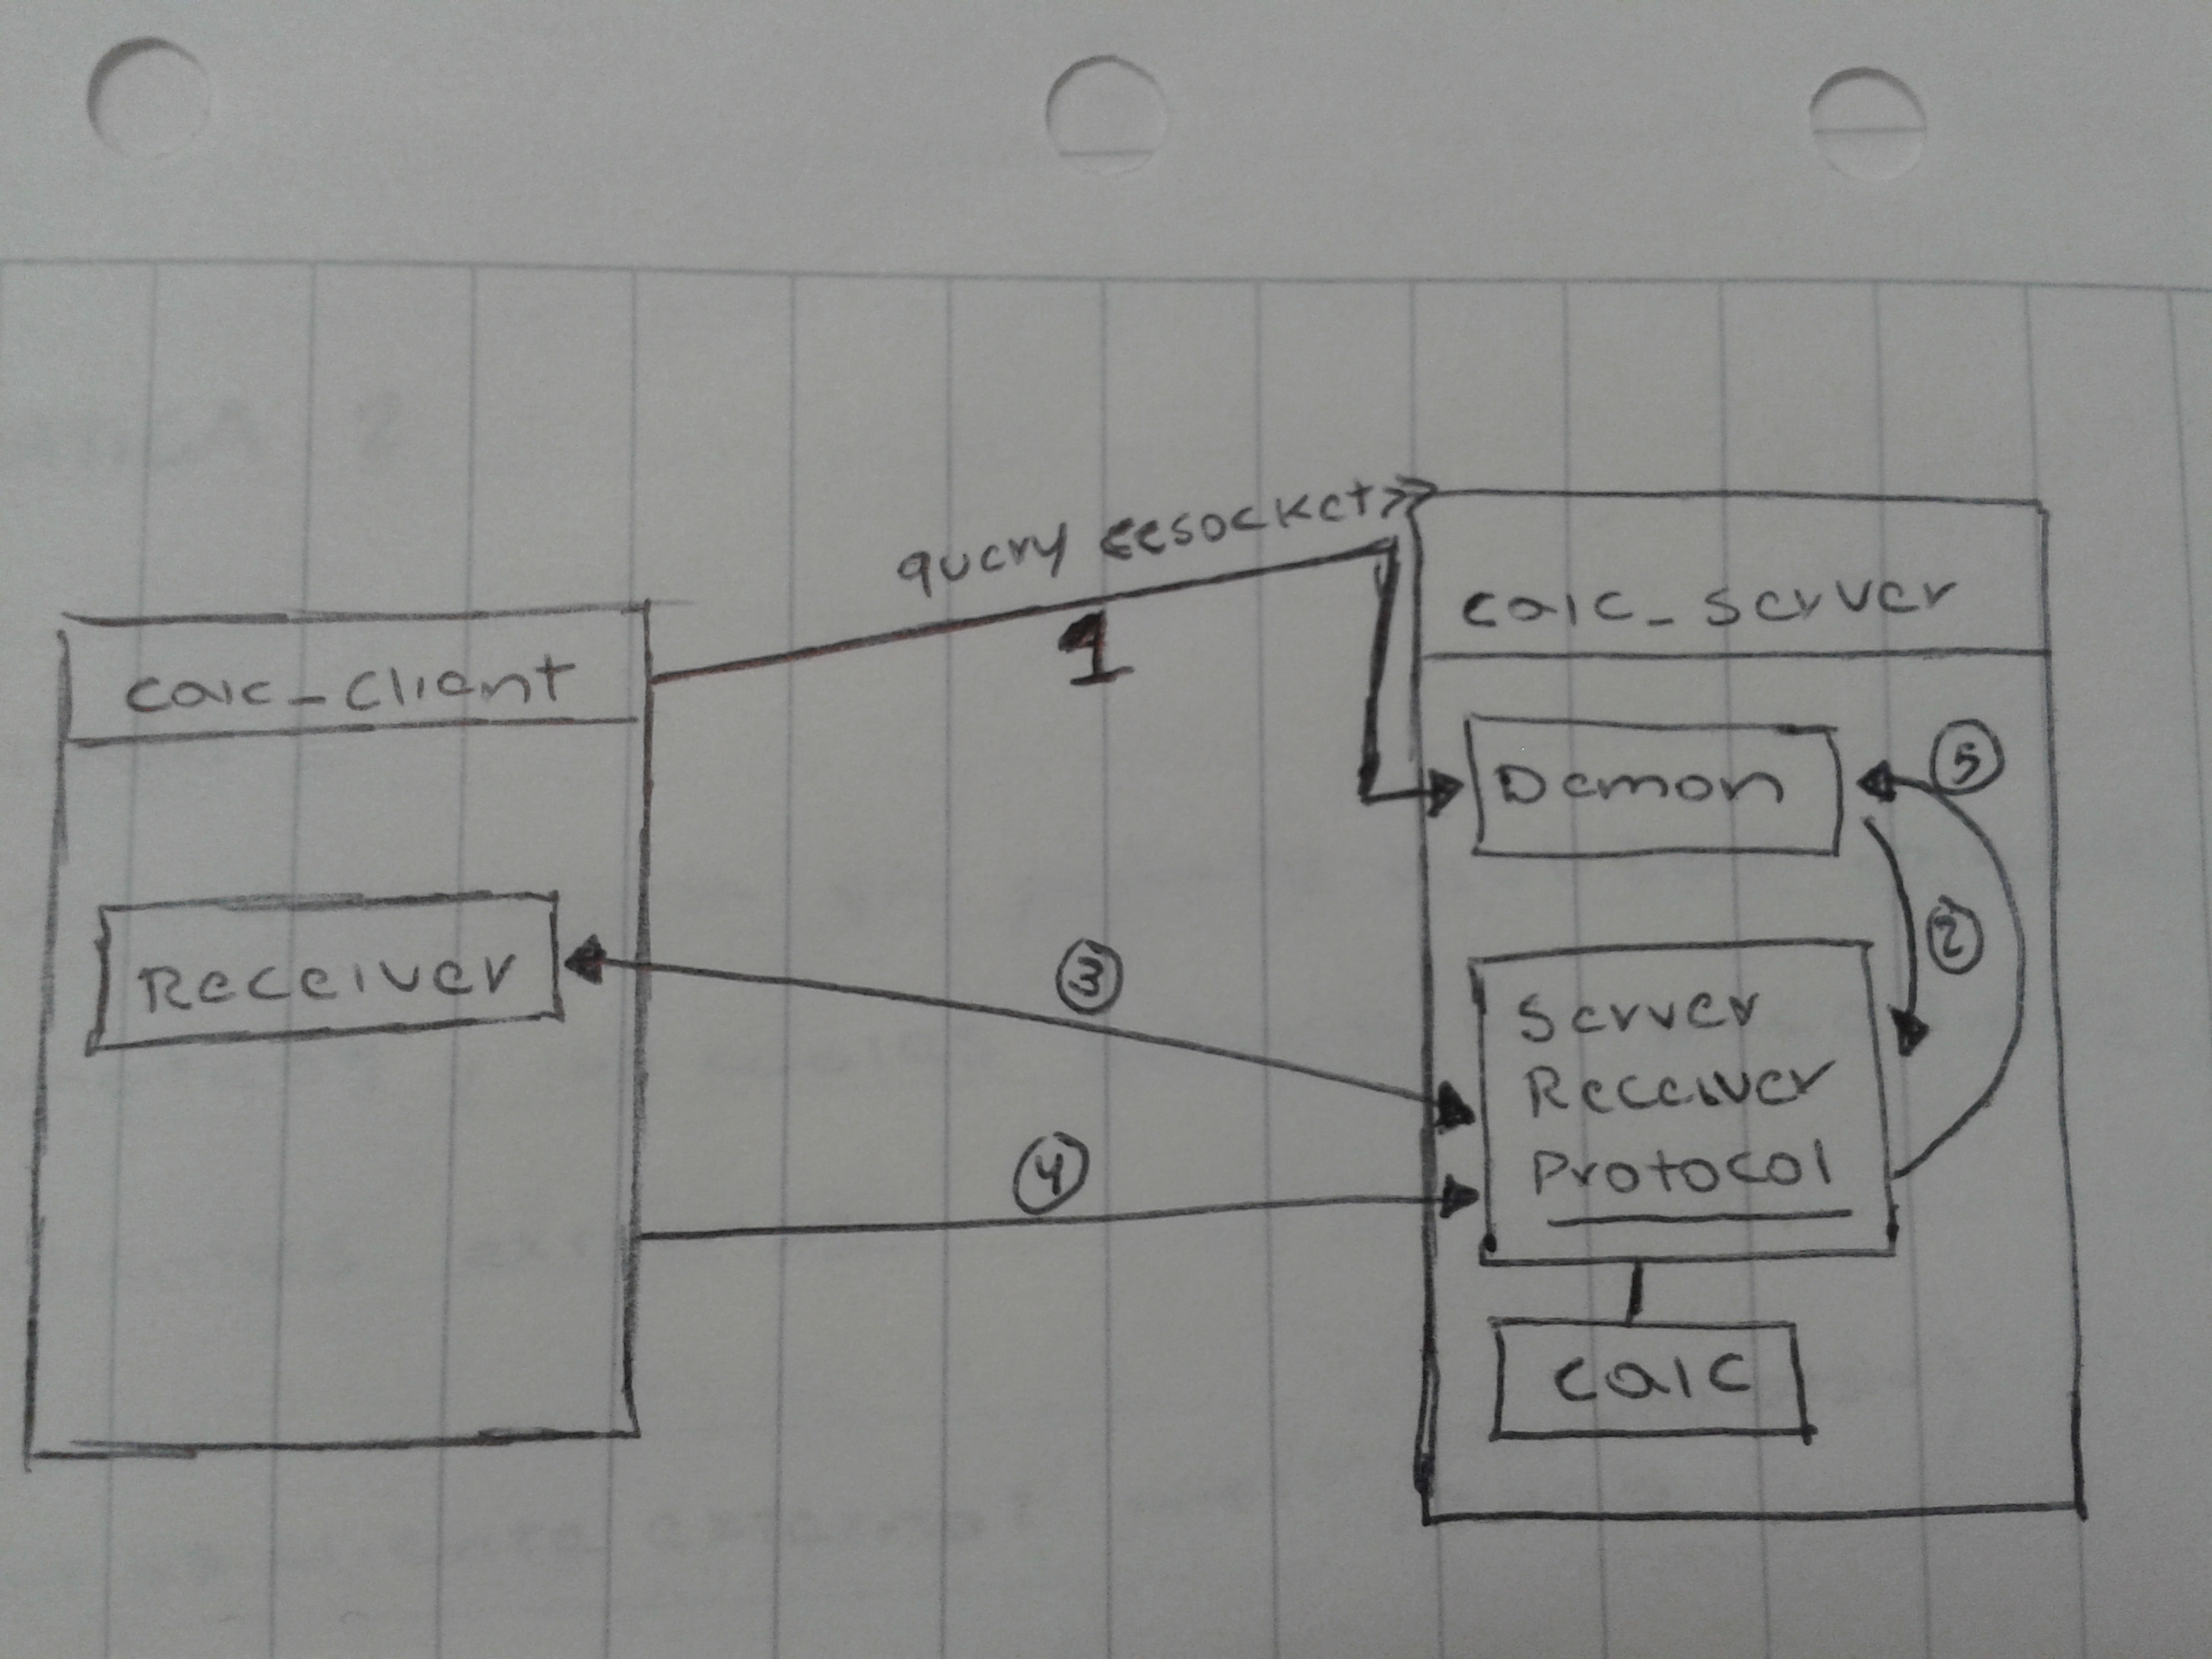
\includegraphics[scale=.1]{tales.jpg}
  
\section{Diseño del Protocolo}

\begin{itemize}
  \item Se trabaja sobre TCP
  \item Define 3 capas
  \item una fisica en la cual se envian y reciben bits
  \item una de comunicacion e interpretacion de la serializacion de los bits
  \item una capa llamada calcular que se encarga de recibir la interpretacion de los bits y hallar un resultado
  \item primera capa comunicacion: es a nivel de sockets y datos serializados con id para cada package
  \item segunda capa comunicacion: es una conexion persistente asi que la comunicacion entre la segunda capa se hace primero con envio de una peticion y luego muchos request
  y response los cuales se pasan en cada caso a la calculadora(capa superior).
  \item tercera capa comunicacion: recibe operaciones procesadas por la segunda capa las interpreta las soluciona y entrega un resultado con sentido logico para el usuario final.
\end{itemize}

\section{Requisitos No Funcionales}
\begin{itemize}
  \item Heterogeneidad
  \item Extensibilidad
  \item Seguridad
  \item Escalabilidad
  \item Tratamiento a fallos
  \item Concurrencia
  \item Transparencia
\end{itemize}

\section{Requisitos No Funcionales}
\begin{itemize}
  \item Heterogeneidad
  \item Extensibilidad
  \item Seguridad
  \item Escalabilidad
  \item Tratamiento a fallos
  \item Concurrencia
  \item Transparencia
\end{itemize}

\section{Implementacion}
  C no tiene clases asi que todo esta separado por metodos, los datos estan serializados con paquete y contenido a nivel de bits, la calculadora en el server hace uso de un sencillo compilador para RPN (Reverse Polish Notacion), para procesar expresiones completas ejemplo: ( 2 + 3 ) * 2, recibe multiples conexiones, para cerrar una conexion se hace uso del comando close, tienen un sistema de validacion de errores y una ayuda a la cual se accede con el comando /?, pero esta no he tenido el tiempo para escribirla :P, sin embargo esta la opcion para acceder a ella.

\end{document}